\documentclass[hyperref={bookmarks=false},aspectratio=169]{beamer}
\usepackage{hyperref,ragged2e,amsmath,amssymb,url,bm}
\usepackage{graphicx,booktabs,array}
\usepackage{tikz}
\usetikzlibrary{arrows.meta,positioning,calc,shapes.geometric,decorations.pathreplacing,matrix}
\graphicspath{{crops/}}
\usetheme{Goettingen}
% --- Paleta de la serie Festividades santas: tierra roja, café rojizo, mostaza y papiro ---
\definecolor{tierraroja}{RGB}{122,40,18}
\definecolor{caferojizo}{RGB}{58,18,8}
\definecolor{mostaza}{RGB}{214,160,58}
\definecolor{papiro}{RGB}{243,228,192}
\definecolor{sepia}{RGB}{98,66,44}
\definecolor{oliva}{RGB}{92,98,48}
\setbeamercolor{structure}{fg=tierraroja}
\setbeamertemplate{sidebar canvas right}[vertical shading][top=tierraroja!92!black,bottom=caferojizo]
\setbeamercolor{title in sidebar}{fg=mostaza}
\setbeamercolor{author in sidebar}{fg=papiro}
\setbeamercolor{section in sidebar}{fg=papiro}
\setbeamercolor{section in sidebar shaded}{fg=mostaza!55!papiro!75!tierraroja}
\setbeamercolor{subsection in sidebar}{fg=papiro}
\setbeamercolor{subsection in sidebar shaded}{fg=mostaza!55!papiro!75!tierraroja}
\let\raggedright\justifying
\setlength{\RaggedRightRightskip}{0pt plus 1fil}
\setbeamertemplate{background canvas}{
\includegraphics[width=\paperwidth,height=\paperheight]{papiro.jpg}}
\setbeamercolor{normal text}{fg=caferojizo!90!black}
\setbeamercolor{frametitle}{fg=tierraroja}
\setbeamerfont{frametitle}{series=\bfseries}
\setbeamertemplate{section in toc shaded}{\leavevmode{\color{sepia!85!black}\inserttocsection}\par}
\setbeamercolor{title}{fg=tierraroja}
\setbeamercolor{subtitle}{fg=sepia}
\setbeamercolor{item projected}{bg=tierraroja,fg=papiro}
\setbeamertemplate{itemize item}{\small\textcolor{mostaza!80!tierraroja}{$\blacktriangleright$}}
\setbeamertemplate{navigation symbols}{}
% --- Español + hebreo + griego (XeLaTeX) con fuentes empaquetadas en fonts/ ---
\usepackage[bidi=default]{babel}
\babelprovide[import,main]{spanish}
\babelprovide[import]{hebrew}
\babelprovide[import]{ancientgreek}
\babelfont[hebrew]{sf}[Path=fonts/, BoldFont=NotoHebrewSans-700.ttf]{NotoHebrewSans-400.ttf}
\babelfont[hebrew]{rm}[Path=fonts/, BoldFont=NotoHebrewSans-700.ttf]{NotoHebrewSans-400.ttf}
\babelfont[ancientgreek]{sf}[Path=fonts/]{GFSPorson.otf}
\babelfont[ancientgreek]{rm}[Path=fonts/]{GFSPorson.otf}
\newcommand{\heb}[1]{\mbox{\foreignlanguage{hebrew}{#1}}}
\newcommand{\grc}[1]{\foreignlanguage{ancientgreek}{#1}}
\newcommand{\SENOR}{S{\fontsize{0.78em}{1em}\selectfont EÑOR}}
% --- Citas, imágenes, referencias ---
\usepackage[most]{tcolorbox}
\newtcolorbox{cita}[1][]{enhanced, colback=papiro, opacityback=0.80, colframe=tierraroja!85!mostaza,
  boxrule=0pt, leftrule=2.5pt, arc=0pt, left=6pt, right=6pt, top=4pt, bottom=4pt,
  before skip=4pt, after skip=6pt, fontupper=\small\itshape, #1}
\newcommand{\fuente}[1]{\par\hfill{\upshape\bfseries\footnotesize\textcolor{tierraroja}{#1}}}
\newcommand{\imagen}[3][0.80]{%
  \centering\includegraphics[height=#1\textheight,width=\linewidth,keepaspectratio]{#2}\par\vspace{2pt}
  {\fontsize{5}{6}\selectfont\color{sepia}{\raggedleft\textit{Nota.} #3\par}}}
\makeatletter
\newcommand{\fotolado}[2]{%
  \begin{tikzpicture}[remember picture,overlay]
    \node[anchor=north east,inner sep=0pt] (foto) at ([xshift=-\beamer@sidebarwidth]current page.north east)
      {\includegraphics[height=\paperheight]{#1}};
    \node[anchor=south east,inner sep=2pt,text=papiro,fill=caferojizo,fill opacity=0.55,text opacity=1,
      font=\fontsize{4.5}{5.5}\selectfont,align=right,text width=4.2cm] at ([xshift=-3pt,yshift=3pt]foto.south east)
      {\textit{Nota.} #2};
  \end{tikzpicture}}
\makeatother
\newcommand{\refapa}[1]{\par{\RaggedRight\hangindent=1.2em\hangafter=1\noindent #1\par}\vspace{3pt}}
\usepackage{xurl}\urlstyle{same}
\newcommand{\destacar}[1]{\textbf{\textcolor{tierraroja}{#1}}}
\newcommand{\precision}[1]{{\footnotesize\color{sepia}\textbf{Precisión:} #1}}
\newcolumntype{L}[1]{>{\RaggedRight\arraybackslash}p{#1}}
\tikzset{caja/.style={draw=tierraroja,line width=0.8pt,fill=papiro,fill opacity=0.90,text opacity=1,rounded corners=3pt,inner sep=5pt,font=\scriptsize}}
\title[Matsot]{\bfseries{Jag haMatsot: la fiesta de los Panes sin Levadura}}
\subtitle{``Celebremos la fiesta\ldots{} con panes sin levadura, de sinceridad y de verdad'' (1 Co 5:8)}
\author{}\institute{}\date{}
\titlegraphic{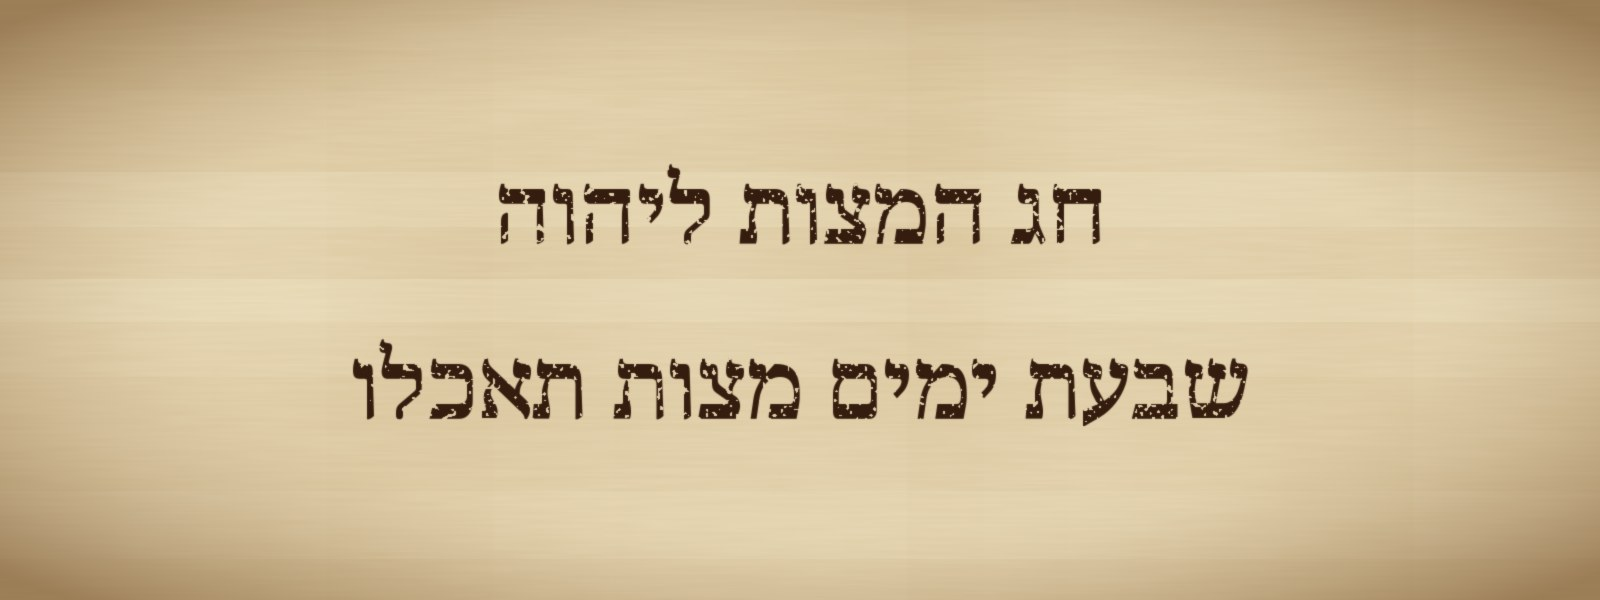
\includegraphics[width=0.80\linewidth,height=0.34\textheight,keepaspectratio]{portada.jpg}\\[-1pt]
  {\fontsize{5}{6}\selectfont\color{sepia}\textit{Nota.} Elaboración propia: Lv 23:6b en texto hebreo consonántico (BHS).}}
\begin{document}
\frame{\titlepage}

\begin{frame}\frametitle{Contenidos}
\begin{columns}[t,onlytextwidth]
\begin{column}{0.48\textwidth}\tableofcontents[sections={1-7}]\end{column}
\begin{column}{0.48\textwidth}\tableofcontents[sections={8-14}]\end{column}
\end{columns}
\end{frame}

% ------------------------------------------------------------------
\section{Introducción}

\begin{frame}{Una semana sin levadura}
\begin{columns}[c,onlytextwidth]
\begin{column}{0.52\textwidth}
\begin{cita}Y guardaréis la fiesta de los panes sin levadura, porque en este mismo día saqué vuestras huestes de la tierra de Egipto\ldots\fuente{(Éx 12:17, RVR1960)}\end{cita}
\small Una fiesta cuyo signo es una \destacar{ausencia}: siete días ``no se hallará levadura en vuestras casas'' (Éx 12:19).
\end{column}
\begin{column}{0.46\textwidth}\small
\begin{itemize}
\item Pascua (14): Israel \destacar{salvado de la muerte}.
\item Ázimos (15--21): Israel \destacar{libre del cautiverio}.
\item Tesis: la fiesta conmemora una salida histórica y enseña una forma de vivir.
\end{itemize}
\precision{distinción de la serie (documento de referencia, lecciones 7 y 11).}
\end{column}
\end{columns}
\end{frame}

\begin{frame}{El lugar en el ciclo}
\centering
\resizebox{\linewidth}{!}{%
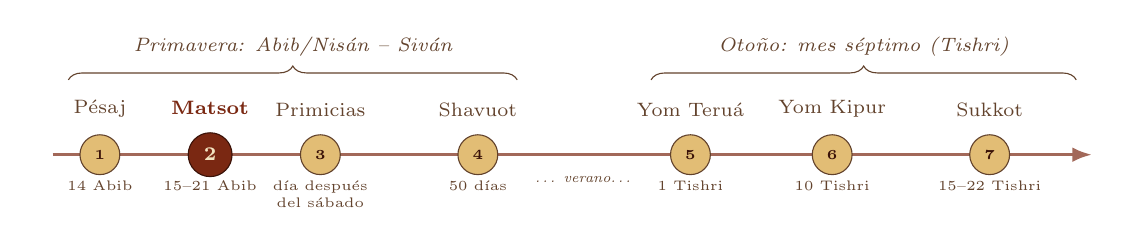
\begin{tikzpicture}[x=1cm,y=1cm,font=\scriptsize]
 \def\fiestaactual{2}
 \draw[line width=1.2pt,tierraroja!70,-{Latex[length=2.5mm]}] (0,0) -- (13.2,0);
 \draw[decorate,decoration={brace,amplitude=5pt},sepia] (0.2,0.95) -- (5.9,0.95) node[midway,above=5pt,font=\scriptsize\itshape]{Primavera: Abib/Nisán -- Siván};
 \draw[decorate,decoration={brace,amplitude=5pt},sepia] (7.6,0.95) -- (13.0,0.95) node[midway,above=5pt,font=\scriptsize\itshape]{Otoño: mes séptimo (Tishri)};
 \foreach \n/\x/\t/\d in {1/0.6/Pésaj/{14 Abib},2/2.0/Matsot/{15--21 Abib},3/3.4/Primicias/{día después del sábado},4/5.4/Shavuot/{50 días},5/8.1/Yom Teruá/{1 Tishri},6/9.9/Yom Kipur/{10 Tishri},7/11.9/Sukkot/{15--22 Tishri}}{
   \ifnum\n=\fiestaactual
     \node[circle,fill=tierraroja,draw=caferojizo,minimum size=5.5mm,text=papiro,font=\scriptsize\bfseries] at (\x,0) {\n};
     \node[above=3pt,font=\scriptsize\bfseries,text=tierraroja] at (\x,0.28) {\t};
   \else
     \node[circle,fill=mostaza!70,draw=sepia,minimum size=4.5mm,text=caferojizo,font=\tiny\bfseries] at (\x,0) {\n};
     \node[above=3pt,text=sepia] at (\x,0.25) {\t};
   \fi
   \node[below=6pt,text width=1.6cm,align=center,font=\tiny,text=sepia] at (\x,0) {\d};}
 \node[font=\tiny\itshape,text=sepia] at (6.75,-0.32) {\ldots\ verano\ldots};
\end{tikzpicture}}\par\medskip
\small La semana que sigue a la Pascua contiene también la gavilla de las \destacar{primicias} (Lv 23:9--14). Sangre que salva, salida que libera, primicia que se presenta.
\end{frame}


% ------------------------------------------------------------------
\section{El texto}

\begin{frame}{Texto ancla: Lv 23:6--8}
\fotolado{panel_levitico23.jpg}{Elaboración propia: Lv 23:6 en texto hebreo consonántico (BHS).}
\begin{columns}[c,onlytextwidth]
\begin{column}{0.57\textwidth}
\begin{cita}Y a los quince días de este mes es la fiesta solemne de los panes sin levadura a \SENOR; siete días comeréis panes sin levadura. El primer día tendréis santa convocación; ningún trabajo de siervos haréis. Y presentaréis a \SENOR{} siete días ofrenda encendida; el séptimo día será santa convocación\ldots\fuente{(Lv 23:6--8, RVR1960)}\end{cita}
\small \heb{חַג הַמַּצּוֹת} (\emph{jag hamatsot}): fiesta de peregrinación ``de las \emph{matsot}''.
\end{column}
\begin{column}{0.41\textwidth}\end{column}
\end{columns}
\end{frame}

\begin{frame}{Una semana entre paréntesis}
\begin{center}\heb{שִׁבְעַת יָמִים מַצּוֹת תֹּאכֵלוּ}\quad {\small ``siete días comeréis \emph{matsot}''}\end{center}
\begin{columns}[t,onlytextwidth]
\begin{column}{0.48\textwidth}\small
\begin{itemize}
\item \destacar{Al centro}: ``siete días'', dos veces (vv.~6, 8).
\item \destacar{En los bordes}: primer y séptimo día con la misma doble fórmula.
\item \heb{מִקְרָא־קֹדֶשׁ} \emph{mikrá kódesh}, ``santa convocación''.
\item \heb{כָּל־מְלֶאכֶת עֲבֹדָה לֹא תַעֲשׂוּ} ``ningún trabajo de siervos''.
\end{itemize}
\end{column}
\begin{column}{0.50\textwidth}
\centering
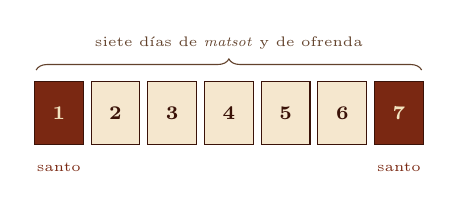
\begin{tikzpicture}[x=0.72cm,font=\scriptsize]
 \foreach \i in {1,...,7}{
   \ifnum\i=1 \def\c{tierraroja}\def\t{papiro}\else\ifnum\i=7 \def\c{tierraroja}\def\t{papiro}\else\def\c{mostaza!25}\def\t{caferojizo}\fi\fi
   \node[draw=caferojizo,fill=\c,text=\t,minimum width=0.62cm,minimum height=0.8cm,font=\scriptsize\bfseries] at (\i,0) {\i};}
 \draw[decorate,decoration={brace,amplitude=4pt},sepia] (0.6,0.55) -- (7.4,0.55) node[midway,above=4pt,font=\tiny]{siete días de \emph{matsot} y de ofrenda};
 \node[below=3pt,font=\tiny,text=tierraroja] at (1,-0.4) {santo};
 \node[below=3pt,font=\tiny,text=tierraroja] at (7,-0.4) {santo};
\end{tikzpicture}\par\medskip
\scriptsize La semana queda encerrada entre dos días santos: una \destacar{inclusión}.
\end{column}
\end{columns}
\end{frame}

\begin{frame}{Las leyes de la fiesta}
\scriptsize\renewcommand{\arraystretch}{1.13}
\begin{tabular}{@{}L{1.9cm}L{2.5cm}L{7.6cm}@{}}
\toprule
\textbf{Texto} & \textbf{Fecha} & \textbf{Qué añade} \\ \midrule
Éx 12:14--20 & 14 tarde -- 21 tarde & ``memoria'', ``estatuto perpetuo''; quitar la \emph{se'or}; \emph{karet}; 1.º y 7.º santos; vale para el extranjero \\
Éx 12:33--39 & la salida & masa ``antes que se leudase''; artesas al hombro; tortas sin levadura \\
Éx 13:3--10 & mes de Abib & ``tened memoria''; nada leudado ``en todo tu territorio''; la instrucción al hijo \\
Éx 23:15; 34:18 & mes de Abib & primera de las tres fiestas de peregrinación \\
Lv 23:6--8 & 15--21 & dentro del calendario completo; ofrenda encendida siete días \\
Nm 28:17--25 & 15--21 & sacrificios diarios: 2 becerros, 1 carnero, 7 corderos, macho cabrío \\
Dt 16:3--4, 8 & ``seis días'' + 7.º & ``pan de aflicción, porque aprisa saliste''; 7.º día \emph{atséret} \\
\bottomrule
\end{tabular}\par\smallskip
\precision{tabla sinóptica de elaboración propia (BHS, RVR1960).}
\end{frame}

\begin{frame}{Pan de aflicción: Dt 16:3}
\fotolado{panel_deuteronomio16.jpg}{Elaboración propia: Dt 16:3 en texto hebreo consonántico (BHS).}
\begin{columns}[c,onlytextwidth]
\begin{column}{0.57\textwidth}
\begin{cita}\ldots{}siete días comerás con ella pan sin levadura, pan de aflicción, porque aprisa saliste de tierra de Egipto; para que todos los días de tu vida te acuerdes del día en que saliste de la tierra de Egipto.\fuente{(Dt 16:3, RVR1960)}\end{cita}
\small \heb{לֶחֶם עֹנִי} \emph{lejem oni}: pan de la \destacar{servidumbre}.\\ \heb{בְחִפָּזוֹן} \emph{bejipazón}: pan de la \destacar{prisa}.\\[2pt]
\scriptsize \emph{Jipazón}: solo Éx 12:11; Dt 16:3; Is 52:12 (``no saldréis apresurados''). Conteo propio.
\end{column}
\begin{column}{0.41\textwidth}\end{column}
\end{columns}
\end{frame}

% ------------------------------------------------------------------
\section{Historia}

\begin{frame}{La prisa de la salida}
\fotolado{panel_exodo12.jpg}{Elaboración propia: Éx 12:39 en texto hebreo consonántico (BHS).}
\begin{columns}[c,onlytextwidth]
\begin{column}{0.57\textwidth}
\begin{cita}Y llevó el pueblo su masa antes que se leudase, sus masas envueltas en sus sábanas sobre sus hombros.\fuente{(Éx 12:34, RVR1960)}\end{cita}
\begin{cita}Y cocieron tortas sin levadura de la masa que habían sacado de Egipto, pues no había leudado, porque al echarlos fuera los egipcios, no habían tenido tiempo ni para prepararse comida.\fuente{(Éx 12:39, RVR1960)}\end{cita}
\scriptsize \heb{מִשְׁאֲרֹתָם} \emph{mish'arotam}: ``sus \destacar{artesas}'' (cf. Éx 8:3 [7:28]). \heb{גֹרְשׁוּ}: ``fueron \destacar{expulsados}''.
\end{column}
\begin{column}{0.41\textwidth}\end{column}
\end{columns}
\end{frame}

\begin{frame}{Pan de pastores, pan de pobres}
\begin{columns}[t,onlytextwidth]
\begin{column}{0.50\textwidth}\small
La \emph{matsá} es el pan rápido: harina, agua y fuego.
\begin{itemize}
\item Abraham: tortas ``de prisa'' (Gn 18:6).
\item Lot: \emph{matsot} para los ángeles (Gn 19:3).
\item Gedeón (Jue 6:19); la mujer de Endor (1 S 28:24).
\end{itemize}
El pan leudado pide tiempo, masa madre y casa estable (Wight, 1953).
\end{column}
\begin{column}{0.48\textwidth}
\begin{tcolorbox}[colback=papiro,colframe=tierraroja,boxrule=1pt,arc=3pt]
\small\centering Comer \emph{matsot} siete días es ponerse en la condición de los que salieron: \destacar{sin casa, sin tiempo, con lo que se carga al hombro}.
\end{tcolorbox}
\precision{la crítica histórica propone un origen agrícola de Matsot distinto del pastoral de Pésaj (de Vaux, 1985; Propp, 1999); el texto da a los ázimos un origen histórico (Éx 12:34, 39).}
\end{column}
\end{columns}
\end{frame}

\begin{frame}{El itinerario de la salida}
\begin{columns}[c,onlytextwidth]
\begin{column}{0.64\textwidth}
\centering
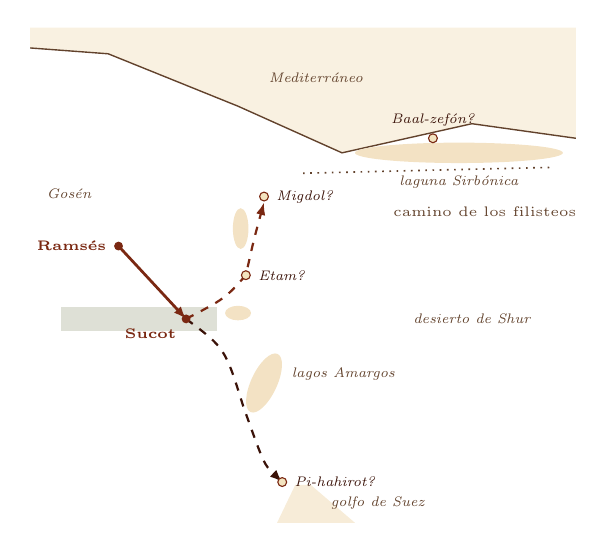
\begin{tikzpicture}[x=3.3cm,y=3.7cm,font=\tiny]
 \fill[mostaza!15] (31.5,31.55) -- (31.5,31.48) -- (31.8,31.46) -- (32.3,31.28) -- (32.7,31.12) -- (33.2,31.22) -- (33.6,31.17) -- (33.6,31.55) -- cycle;
 \draw[sepia,line width=0.5pt] (31.5,31.48) -- (31.8,31.46) -- (32.3,31.28) -- (32.7,31.12) -- (33.2,31.22) -- (33.6,31.17);
 \node[font=\tiny\itshape,text=sepia] at (32.6,31.38) {Mediterráneo};
 \fill[mostaza!30] (33.15,31.12) ellipse (0.40 and 0.035);
 \fill[mostaza!30] (32.31,30.86) ellipse (0.03 and 0.07);
 \fill[mostaza!30] (32.30,30.57) ellipse (0.05 and 0.025);
 \fill[mostaza!30,rotate around={-25:(32.40,30.33)}] (32.40,30.33) ellipse (0.05 and 0.11);
 \fill[mostaza!20] (32.52,29.98) -- (32.58,29.98) -- (32.75,29.85) -- (32.45,29.85) -- cycle;
 \node[font=\tiny\itshape,text=sepia,anchor=west] at (32.62,29.92) {golfo de Suez};
 \node[font=\tiny\itshape,text=sepia,anchor=west] at (32.47,30.36) {lagos Amargos};
 \node[font=\tiny\itshape,text=sepia] at (33.15,31.02) {laguna Sirbónica};
 \node[font=\tiny\itshape,text=sepia] at (31.65,30.98) {Gosén};
 \node[font=\tiny\itshape,text=sepia] at (33.2,30.55) {desierto de Shur};
 \fill[oliva!20] (31.62,30.51) rectangle (32.22,30.59);
 \draw[sepia,dotted,line width=0.6pt] (32.55,31.05) -- (33.5,31.07);
 \node[font=\tiny,text=sepia] at (33.25,30.92) {camino de los filisteos};
 \draw[tierraroja,line width=1pt,-{Latex[length=1.6mm]}] (31.84,30.80) -- (32.10,30.55);
 \draw[tierraroja,line width=0.8pt,dashed,-{Latex[length=1.6mm]}] (32.10,30.55) .. controls (32.25,30.62) .. (32.33,30.70) .. controls (32.36,30.82) .. (32.40,30.95);
 \draw[caferojizo,line width=0.8pt,dashed,-{Latex[length=1.6mm]}] (32.10,30.55) .. controls (32.25,30.45) .. (32.32,30.25) .. controls (32.40,30.05) .. (32.47,29.99);
 \fill[tierraroja] (31.84,30.80) circle (1.6pt) node[left=1pt,font=\tiny\bfseries,text=tierraroja]{Ramsés};
 \fill[tierraroja] (32.10,30.55) circle (1.6pt) node[below left=0pt,font=\tiny\bfseries,text=tierraroja]{Sucot};
 \foreach \x/\y/\n/\p in {32.33/30.70/{Etam?}/right, 32.40/30.97/{Migdol?}/right, 32.47/29.99/{Pi-hahirot?}/right, 33.05/31.17/{Baal-zefón?}/above}{
   \draw[tierraroja,fill=papiro] (\x,\y) circle (1.6pt); \node[\p=1pt,font=\tiny\itshape,text=caferojizo] at (\x,\y) {\n};}
\end{tikzpicture}
\end{column}
\begin{column}{0.34\textwidth}\scriptsize
Ramsés $\rightarrow$ Sucot $\rightarrow$ Etam $\rightarrow$ vuelta a Pi-hahirot, ``entre Migdol y el mar'' (Éx 12:37; 13:20; 14:2; Nm 33:3--8).\par\medskip
\tikz\draw[tierraroja,dashed,line width=0.8pt] (0,0)--(0.5,0); ruta norte\\
\tikz\draw[caferojizo,dashed,line width=0.8pt] (0,0)--(0.5,0); ruta sur\par\medskip
\precision{mapa esquemático; los lugares con ``?'' tienen identificación discutida (Hoffmeier, 1997; Kitchen, 2003).}
\end{column}
\end{columns}
\end{frame}


\begin{frame}{¿Cuándo cruzaron el mar?}
\scriptsize\renewcommand{\arraystretch}{1.1}
\begin{tabular}{@{}L{0.9cm}L{3.5cm}L{3.9cm}L{3.6cm}@{}}
\toprule
\textbf{Abib} & \textbf{Serie} & \textbf{Texto explícito} & \textbf{Tradición rabínica} \\ \midrule
15 & salida; Sucot & única fecha: Nm 33:3 & salida \\
16 & Etam & Etam (13:20), sin fecha & marcha \\
17 & Migdol, ``al tercer día''; cruce & alcanzados ``junto al mar'' (14:9), sin fecha & fin de los tres días (Éx 3:18) \\
18 & ``libres del faraón'', primicia & --- & aviso al faraón (Rashi a Éx 14:5) \\
19--20 & --- & --- & persecución \\
21 & 7.º día santo & \emph{mikrá kódesh} (Lv 23:8) & cruce de noche; Cántico \\
\bottomrule
\end{tabular}\par\medskip
\precision{ambas cronologías completas son reconstrucciones. Josefo hace llegar a Israel a Beelsefón ``al tercer día'' (Ant. 2.315; verificar). El texto dice que el cruce fue de noche (Éx 14:21) y que siguieron ``tres días'' hasta Mara (15:22).}
\end{frame}

\begin{frame}{La semana y los hechos de la salida}
\centering
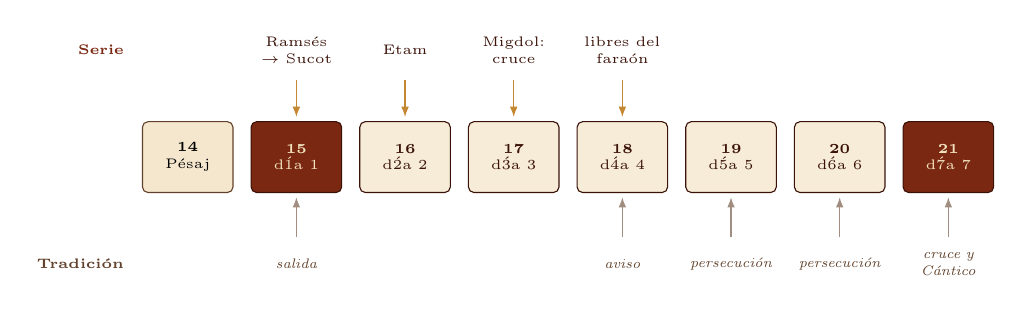
\begin{tikzpicture}[x=1.38cm,y=0.85cm,font=\tiny]
 \node[draw=sepia,fill=mostaza!25,minimum width=1.15cm,minimum height=0.9cm,align=center,rounded corners=2pt] at (0,0) {\textbf{14}\\Pésaj};
 \foreach \i/\d in {1/15,2/16,3/17,4/18,5/19,6/20,7/21}{
   \ifnum\i=1 \def\col{tierraroja}\def\tx{papiro}\else\ifnum\i=7 \def\col{tierraroja}\def\tx{papiro}\else\def\col{mostaza!20}\def\tx{caferojizo}\fi\fi
   \node[draw=caferojizo,fill=\col,text=\tx,minimum width=1.15cm,minimum height=0.9cm,align=center,rounded corners=2pt] (d\i) at (\i,0) {\textbf{\d}\\día \i};}
 \node[font=\tiny\bfseries,text=tierraroja,anchor=east] at (-0.5,1.6) {Serie};
 \foreach \i/\t in {1/{Ramsés $\rightarrow$ Sucot},2/{Etam},3/{Migdol: cruce},4/{libres del faraón}}{
   \node[text width=1.2cm,align=center,text=caferojizo] at (\i,1.6) {\t};
   \draw[mostaza!80!tierraroja,-{Latex[length=1.3mm]}] (\i,1.15) -- (\i,0.6);}
 \node[font=\tiny\bfseries,text=sepia,anchor=east] at (-0.5,-1.6) {Tradición};
 \foreach \i/\t in {1/{salida},4/{aviso},5/{persecución},6/{persecución},7/{cruce y Cántico}}{
   \node[text width=1.2cm,align=center,font=\tiny\itshape,text=sepia] at (\i,-1.6) {\t};
   \draw[sepia!60,-{Latex[length=1.3mm]}] (\i,-1.2) -- (\i,-0.6);}
\end{tikzpicture}\par\medskip
\small En rojo, los dos días de \emph{mikrá kódesh}. La sinagoga lee el Cántico del Mar (Éx 15) el séptimo día (Meguilá 31a).\par
\precision{lectura de la serie frente a Rashi a Éx 14:5 y Seder Olam.}
\end{frame}

\begin{frame}{La fecha del éxodo}
\begin{columns}[c,onlytextwidth]
\begin{column}{0.56\textwidth}
\centering
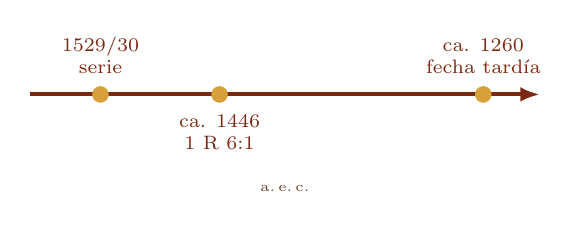
\begin{tikzpicture}[x=-0.018cm,font=\scriptsize]
 \draw[line width=1.4pt,tierraroja,-{Latex[length=2.5mm]}] (1580,0) -- (1220,0);
 \foreach \a/\t/\s in {1530/{1529/30\\serie}/1,1446/{ca. 1446\\1 R 6:1}/-1,1260/{ca. 1260\\fecha tardía}/1}{
  \fill[mostaza] (\a,0) circle (3pt);
  \ifnum\s=1 \node[above=4pt,align=center,text=tierraroja] at (\a,0) {\t};\else\node[below=4pt,align=center,text=tierraroja] at (\a,0) {\t};\fi}
 \node[font=\tiny,text=sepia] at (1400,-1.2) {a.\,e.\,c.};
\end{tikzpicture}
\end{column}
\begin{column}{0.42\textwidth}\scriptsize
\begin{itemize}
\item \destacar{Serie}: 1529/1530 a.\,e.\,c., cómputo propio.
\item \destacar{1 R 6:1}: 480 años hasta el 4.º año de Salomón (ca. 966) $\Rightarrow$ ca. 1446.
\item \destacar{Fecha tardía}: ca. 1260, Ramsés II (Éx 1:11; Kitchen, 2003).
\end{itemize}
\precision{el 15 de Abib es el mismo en cualquier hipótesis. Éx 12:40: LXX y Samaritano añaden ``y en Canaán'' (cf. Gá 3:17).}
\end{column}
\end{columns}
\end{frame}

\begin{frame}{La fiesta en la historia}
\centering
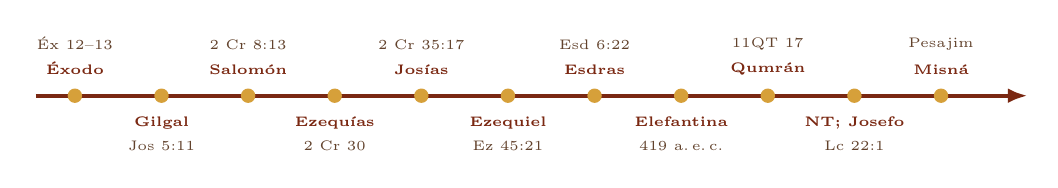
\begin{tikzpicture}[x=1cm,font=\tiny]
 \draw[line width=1.5pt,tierraroja,-{Latex[length=2.5mm]}] (-0.3,0) -- (12.3,0);
 \foreach \x/\a/\b/\s in {0.2/{Éxodo}/{Éx 12--13}/1, 1.3/{Gilgal}/{Jos 5:11}/-1, 2.4/{Salomón}/{2 Cr 8:13}/1, 3.5/{Ezequías}/{2 Cr 30}/-1, 4.6/{Josías}/{2 Cr 35:17}/1, 5.7/{Ezequiel}/{Ez 45:21}/-1, 6.8/{Esdras}/{Esd 6:22}/1, 7.9/{Elefantina}/{419 a.\,e.\,c.}/-1, 9.0/{Qumrán}/{11QT 17}/1, 10.1/{NT; Josefo}/{Lc 22:1}/-1, 11.2/{Misná}/{Pesajim}/1}{
   \fill[mostaza] (\x,0) circle (2.6pt);
   \ifnum\s=1
     \node[above=4pt,font=\tiny\bfseries,text=tierraroja] at (\x,0) {\a};
     \node[above=13pt,font=\tiny,text=sepia] at (\x,0) {\b};
   \else
     \node[below=4pt,font=\tiny\bfseries,text=tierraroja] at (\x,0) {\a};
     \node[below=13pt,font=\tiny,text=sepia] at (\x,0) {\b};
   \fi}
\end{tikzpicture}\par\medskip
\small\begin{itemize}
\item \destacar{Ezequías}: mes segundo, y ``otros siete días'' (2 Cr 30:13, 23). \destacar{Esdras}: ``con regocijo'' (Esd 6:22).
\item \destacar{Elefantina}: carta que ordena guardar 15--21 de Nisán sin leudado (Porten, 1968).
\item \destacar{Siglo I}: ``la fiesta de los panes sin levadura, que se llama la pascua'' (Lc 22:1); Josefo: ``que llamamos Pascua'' (Ant. 14.21).
\end{itemize}
\end{frame}


% ------------------------------------------------------------------
\section{Filología}

\begin{frame}{Cuatro palabras para la masa}
\scriptsize\renewcommand{\arraystretch}{1.15}
\begin{tabular}{@{}L{2.4cm}L{3.0cm}L{6.6cm}@{}}
\toprule
\textbf{Palabra} & \textbf{Sentido} & \textbf{Textos y notas} \\ \midrule
\heb{מַצָּה} \emph{matsá} & torta sin leudar & 53 veces en 42 vv. (conteo propio); etimología discutida (BDB; ¿gr. \grc{μᾶζα}?) \\
\heb{חָמֵץ} \emph{jamets} & lo leudado & 13 veces; raíz ``agriarse'': \emph{jómets} = vinagre (Sal 69:21 [69:22]); ``se agrió mi corazón'' (Sal 73:21) \\
\heb{שְׂאֹר} \emph{se'or} & masa madre, la levadura misma & 5 veces: Éx 12:15, 19; 13:7; Lv 2:11; Dt 16:4 \\
\heb{מַחְמֶצֶת} \emph{majméset} & cualquier cosa leudada & solo Éx 12:19--20 \\
\bottomrule
\end{tabular}\par\medskip
\small Éx 12:15: \heb{תַּשְׁבִּיתוּ שְׂאֹר מִבָּתֵּיכֶם}, ``haréis \destacar{cesar} la masa madre'': hifil de \heb{שׁבת}, la raíz de \emph{shabat}.\par
\precision{conteos propios con la BHS y números Strong; verificar en e-Sword.}
\end{frame}

\begin{frame}{\emph{Karet}: ``será cortado''}
\begin{columns}[t,onlytextwidth]
\begin{column}{0.46\textwidth}
\centering\heb{וְנִכְרְתָה הַנֶּפֶשׁ הַהִוא מִיִּשְׂרָאֵל}
\begin{cita}\ldots{}cualquiera que comiere leudado desde el primer día hasta el séptimo, será cortado de Israel.\fuente{(Éx 12:15, RVR1960)}\end{cita}
\end{column}
\begin{column}{0.52\textwidth}\scriptsize
\begin{enumerate}
\item Muerte prematura por mano de Dios (Wenham, 1979).
\item Extinción de la descendencia; exclusión de los antepasados (Milgrom, 1991).
\item Exclusión de la comunidad.
\item Rabínica: castigo divino; 36 transgresiones, entre ellas comer \emph{jamets} en Pésaj (Keritot 1:1).
\end{enumerate}
\precision{el sentido de \emph{karet} es debatido.}
\end{column}
\end{columns}
\end{frame}

\begin{frame}{Las palabras del marco}
\scriptsize\renewcommand{\arraystretch}{1.15}
\begin{tabular}{@{}L{2.7cm}L{9.3cm}@{}}
\toprule
\heb{לֶחֶם עֹנִי} \emph{lejem oni} & ``pan de aflicción''; raíz de la opresión (Éx 1:11; 3:7) y del ayuno (Lv 16:29) \\
\heb{מִקְרָא קֹדֶשׁ} & ``santa convocación'' (``citación santa'', serie); LXX \grc{κλητὴ ἁγία} \\
\heb{עֲצֶרֶת} \emph{atséret} & ``asamblea de clausura'': 7.º día (Dt 16:8; LXX \grc{ἐξόδιον}) y 8.º de Sukkot (Lv 23:36) \\
\heb{צִבְאוֹתֵיכֶם} & ``vuestras huestes'' (RVR1960; ``ejércitos'' RV1909): Israel sale en orden (Éx 12:17, 41, 51; 13:18) \\
\heb{בְּעֶצֶם הַיּוֹם הַזֶּה} & ``en el hueso de este día'': Éx 12:17, 41, 51; Jos 5:11 (conteo propio) \\
\bottomrule
\end{tabular}\par\medskip
\small El pueblo sale como \destacar{hueste del \SENOR} en el \destacar{día exacto}: la fiesta guarda la fecha.
\end{frame}

\begin{frame}{Del hebreo al español}
\centering
\begin{tikzpicture}[node distance=0.45cm,font=\scriptsize]
 \node[caja,text width=2.2cm,align=center] (h) {\textbf{Hebreo}\\ \heb{שְׂאֹר} \emph{se'or}\\ \heb{חָמֵץ} \emph{jamets}\\ \heb{מַצּוֹת} \emph{matsot}};
 \node[caja,text width=2.2cm,align=center,right=of h] (l) {\textbf{LXX}\\ \grc{ζύμη}\\ \grc{ζυμωτόν}\\ \grc{ἄζυμα}};
 \node[caja,text width=2.2cm,align=center,right=of l] (n) {\textbf{NT}\\ \grc{ζύμη}\\ \grc{νέον φύραμα}\\ \grc{ἄζυμοι}};
 \node[caja,text width=2.2cm,align=center,right=of n,fill=tierraroja,text=papiro] (e) {\textbf{Español}\\ levadura\\ masa nueva\\ sin levadura};
 \foreach \a/\b in {h/l,l/n,n/e} \draw[-{Latex[length=2.5mm]},mostaza!90!tierraroja,line width=1.3pt] (\a)--(\b);
\end{tikzpicture}\par\medskip
\small\itshape\color{sepia} De la masa madre que se guarda a la ``levadura vieja'' que se limpia (1 Co 5:7).
\end{frame}

\begin{frame}{El griego de la fiesta}
\scriptsize\renewcommand{\arraystretch}{1.15}
\begin{tabular}{@{}L{3.1cm}L{8.9cm}@{}}
\toprule
\grc{τὰ ἄζυμα} & los días de la fiesta: Mc 14:1, 12; Lc 22:1, 7; Hch 12:3; 20:6 \\
\grc{ἄζυμοι} & ``sin levadura como sois'' (1 Co 5:7): \destacar{personas} ázimas \\
\grc{ζύμη} & ``un poco de levadura leuda toda la masa'' (1 Co 5:6; Gá 5:9); ``de los fariseos'' (Mt 16:6) \\
\grc{νέον φύραμα} & ``masa nueva''; \grc{φύραμα} también en Nm 15:20 LXX y Ro 11:16 \\
\grc{εἰλικρίνεια} & ``sinceridad'', pureza sin mezcla (etimología ``juzgado al sol'': popular, insegura) \\
\grc{ἀλήθεια} & ``verdad''; en la LXX traduce \emph{emet} \\
\bottomrule
\end{tabular}
\end{frame}

% ------------------------------------------------------------------
\section{Texto}

\begin{frame}{Problemas de cómputo}
\begin{columns}[t,onlytextwidth]
\begin{column}{0.49\textwidth}\scriptsize
\destacar{``El primer día'' (Éx 12:15).} La levadura debe estar fuera antes de la cena del 14 por la tarde (12:8, 18). Rabínica: \emph{aj} limita al mediodía del 14 (Pesajim 5a).\par\medskip
\destacar{``Seis días'' (Dt 16:8).} (1) Seis tras la noche de Pésaj (Tigay, 1996); (2) patrón ``seis\ldots{} y el séptimo''; (3) rabínica: solo la 1.ª noche obliga a comer \emph{matsá} (Pesajim 120a).
\end{column}
\begin{column}{0.49\textwidth}\scriptsize
\destacar{Mc 14:12.} \grc{τῇ πρώτῃ ἡμέρᾳ τῶν ἀζύμων, ὅτε τὸ πάσχα ἔθυον}: uso popular que cuenta el 14 como primer día (Josefo, \emph{Guerra} 5.99; Ant. 2.317).\par\medskip
\begin{tcolorbox}[colback=papiro,colframe=mostaza!80!tierraroja,boxrule=0.8pt,arc=2pt,left=3pt,right=3pt,top=2pt,bottom=2pt]
\textbf{Precisión textual.} Éx 12:17 TM ``guardaréis las \emph{matsot}''; LXX \grc{τὴν ἐντολὴν ταύτην}, ``este mandamiento'' (¿\heb{הַמִּצְוָה}?). Ez 45:21 TM ``semanas''; LXX ``siete días''.
\end{tcolorbox}
\end{column}
\end{columns}
\end{frame}

\begin{frame}{La levadura en las ofrendas}
\scriptsize\renewcommand{\arraystretch}{1.13}
\begin{tabular}{@{}L{2.2cm}L{5.0cm}L{4.8cm}@{}}
\toprule
\textbf{Texto} & \textbf{Norma} & \textbf{Observación} \\ \midrule
Lv 2:11 & ninguna ofrenda quemada con levadura ni miel & regla del altar (el documento cita 2:4--5) \\
Lv 6:17 [6:10] & la porción sacerdotal ``no se cocerá con levadura'' & santísima \\
Éx 23:18; 34:25 & no ofrecer con pan leudo la sangre & sacrificio \\
Lv 7:13 & acción de gracias con ``tortas de pan leudo'' & se comen, no se queman \\
Lv 23:17 & Shavuot: dos panes ``cocidos con levadura'' & ``no subirán sobre el altar'' (Lv 2:12) \\
\bottomrule
\end{tabular}\par\medskip
\small La levadura está excluida del \destacar{altar} y de la \destacar{fiesta}, no de la \destacar{mesa}. La serie lee los dos panes de Shavuot como los pueblos aún con pecado, presentados para su redención.
\end{frame}

% ------------------------------------------------------------------
\section{Literatura}

\begin{frame}{La ley dentro del relato (Éx 12--13)}
\centering
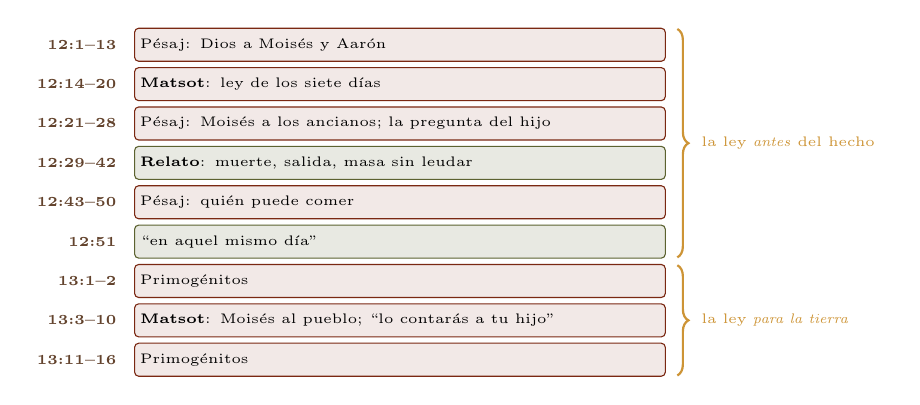
\begin{tikzpicture}[x=1cm,y=-0.5cm,font=\tiny]
 \tikzset{ley/.style={draw=tierraroja,fill=tierraroja!10,rounded corners=1.5pt,text width=6.6cm,inner sep=2pt,minimum height=0.42cm},
          rel/.style={draw=oliva,fill=oliva!14,rounded corners=1.5pt,text width=6.6cm,inner sep=2pt,minimum height=0.42cm}}
 \foreach \y/\r/\t/\s in {0/{12:1--13}/{Pésaj: Dios a Moisés y Aarón}/ley, 1/{12:14--20}/{\textbf{Matsot}: ley de los siete días}/ley, 2/{12:21--28}/{Pésaj: Moisés a los ancianos; la pregunta del hijo}/ley, 3/{12:29--42}/{\textbf{Relato}: muerte, salida, masa sin leudar}/rel, 4/{12:43--50}/{Pésaj: quién puede comer}/ley, 5/{12:51}/{``en aquel mismo día''}/rel, 6/{13:1--2}/{Primogénitos}/ley, 7/{13:3--10}/{\textbf{Matsot}: Moisés al pueblo; ``lo contarás a tu hijo''}/ley, 8/{13:11--16}/{Primogénitos}/ley}{
   \node[\s,anchor=west] at (1.5,\y) {\t};
   \node[anchor=east,font=\tiny\bfseries,text=sepia] at (1.4,\y) {\r};}
 \draw[decorate,decoration={brace,amplitude=4pt},mostaza!90!tierraroja,line width=0.8pt] (8.4,-0.4) -- (8.4,5.4) node[midway,right=5pt,text width=2.3cm]{la ley \emph{antes} del hecho};
 \draw[decorate,decoration={brace,amplitude=4pt},mostaza!90!tierraroja,line width=0.8pt] (8.4,5.6) -- (8.4,8.4) node[midway,right=5pt,text width=2.3cm]{la ley \emph{para la tierra}};
\end{tikzpicture}\par\smallskip
\scriptsize La ley anticipa, el relato prueba, la ley recuerda. En el centro, la catequesis familiar: ``¿Qué es este rito vuestro?'' (12:26; 13:8).
\end{frame}


\begin{frame}{Lot y Abraham (Gn 18--19)}
\begin{columns}[t,onlytextwidth]
\begin{column}{0.50\textwidth}\small
\destacar{Lectura de la serie}: Lot ofrece panes sin levadura (\heb{וּמַצּוֹת אָפָה}, Gn 19:3) porque era la fiesta; Abraham no (Gn 18:6--8), ``porque no era aún época de consumirlos''. La ley existía en el ``período tácito''.
\end{column}
\begin{column}{0.48\textwidth}\scriptsize
\precision{Rashi a Gn 19:3: ``era Pésaj''; pero la tradición sitúa también en Pésaj la visita a Abraham. El texto no dice que las \emph{ugot} de Sara llevaran levadura; ambas escenas son del mismo día (Gn 19:1). La \emph{matsá} era pan de hospitalidad apurada (Jue 6:19; 1 S 28:24). Lectura posible como eco, no explícita.}
\end{column}
\end{columns}
\end{frame}

\begin{frame}{La levadura en la Biblia}
\centering
\begin{tikzpicture}[font=\scriptsize]
 \node[draw=caferojizo,line width=1pt,fill=papiro,circle,minimum size=1.7cm,align=center,font=\scriptsize\bfseries,text=tierraroja] (c) at (0,0) {Levadura\\ \grc{ζύμη}};
 \node[caja,text width=4.2cm,anchor=east] (n) at (-1.4,0.95) {\textbf{\textcolor{tierraroja}{Lo que corrompe}}\\ doctrina (Mt 16:6, 12); hipocresía (Lc 12:1); Herodes (Mc 8:15); malicia (1 Co 5:8); Gá 5:9};
 \node[caja,text width=4.2cm,anchor=west,draw=oliva] (p) at (1.4,0.95) {\textbf{\textcolor{oliva!80!black}{Lo que crece}}\\ el reino, en ``tres medidas de harina'' (Mt 13:33; cf. Gn 18:6)};
 \node[caja,text width=4.2cm,anchor=east,draw=sepia] (a) at (-1.4,-1.0) {\textbf{\textcolor{sepia}{Fuera del altar y de la fiesta}}\\ Lv 2:11; 6:17; Éx 12:15--20};
 \node[caja,text width=4.2cm,anchor=west,draw=sepia] (b) at (1.4,-1.0) {\textbf{\textcolor{sepia}{Ordenada en la mesa}}\\ Lv 7:13; 23:17};
 \foreach \x in {n,p,a,b} \draw[mostaza!90!tierraroja,line width=1pt] (c) -- (\x);
\end{tikzpicture}\par\medskip
\small La Biblia interpreta la Biblia: la levadura significa \destacar{lo que se esparce}; el contexto dice si es malicia o reino.
\end{frame}


\begin{frame}{Cuatro levaduras en el NT}
\centering
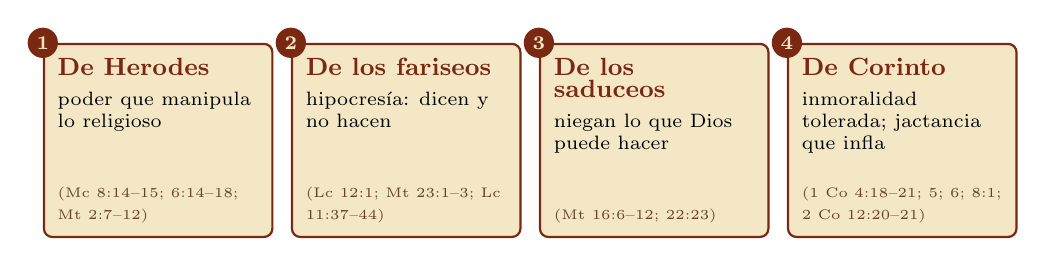
\begin{tikzpicture}
 \foreach \x/\n/\t/\d/\r in {0/1/{De Herodes}/{poder que manipula lo religioso}/{Mc 8:14--15; 6:14--18; Mt 2:7--12}, 3.15/2/{De los fariseos}/{hipocresía: dicen y no hacen}/{Lc 12:1; Mt 23:1--3; Lc 11:37--44}, 6.3/3/{De los saduceos}/{niegan lo que Dios puede hacer}/{Mt 16:6--12; 22:23}, 9.45/4/{De Corinto}/{inmoralidad tolerada; jactancia que infla}/{1 Co 4:18--21; 5; 6; 8:1; 2 Co 12:20--21}}{
  \node[caja,anchor=north] (b\n) at (\x,0) {\parbox[t][2.1cm][t]{2.55cm}{\RaggedRight
    {\small\textbf{\textcolor{tierraroja}{\t}}}\\[3pt]\scriptsize \d\par\vfill{\tiny\color{sepia}(\r)}}};
  \node[circle,fill=tierraroja,text=papiro,font=\scriptsize\bfseries,inner sep=1.6pt] at (b\n.north west) {\n};}
\end{tikzpicture}\par\medskip
\small Lo común: algo que entra y \destacar{infla} la masa desde dentro (\grc{φυσιόω}, ``envanecer'', 1 Co 4:18; 5:2; 8:1).\par
\scriptsize\color{sepia} Esquema de la presentación de Danilo, ``Los Panes sin Levadura''. Eco de raíz: \heb{חֲמוּץ בְּגָדִים} ``vestidos rojos'' (Is 63:1; cf. Ap 19:13).
\end{frame}

\begin{frame}{1 Co 5:6--8: el argumento}
\fotolado{panel_1corintios5.jpg}{Elaboración propia: 1 Co 5:7b--8a en escritura uncial (texto NA28).}
\begin{columns}[c,onlytextwidth]
\begin{column}{0.57\textwidth}
\begin{cita}\ldots{}Limpiaos, pues, de la vieja levadura, para que seáis nueva masa, sin levadura como sois; porque nuestra pascua, que es Cristo, ya fue sacrificada por nosotros. Así que celebremos la fiesta, no con la vieja levadura, ni con la levadura de malicia y de maldad, sino con panes sin levadura, de sinceridad y de verdad.\fuente{(1 Co 5:7--8, RVR1960)}\end{cita}
\scriptsize \grc{καὶ γὰρ τὸ πάσχα ἡμῶν ἐτύθη Χριστός}: el \destacar{sacrificio precede} a la limpieza.
\end{column}
\begin{column}{0.41\textwidth}\end{column}
\end{columns}
\end{frame}

\begin{frame}{Estructura de 1 Co 5:6--8}
\centering
\begin{tikzpicture}[node distance=0.16cm,font=\scriptsize]
 \tikzset{b/.style={draw=tierraroja,fill=papiro,fill opacity=0.9,text opacity=1,rounded corners=2pt,text width=7.6cm,inner sep=3pt},
          lab/.style={fill=tierraroja,text=papiro,font=\tiny\bfseries,rounded corners=1.5pt,text width=1.8cm,align=center,inner sep=2pt}}
 \node[b] (a) {``Un poco de levadura leuda toda la masa'': el contagio};
 \node[b,below=of a] (b2) {\grc{ἐκκαθάρατε} ``limpiaos'' (aoristo): limpieza decisiva; ``nueva masa''};
 \node[b,below=of b2] (c) {\grc{καθώς ἐστε ἄζυμοι} ``sin levadura como sois''};
 \node[b,below=of c,fill=tierraroja!12] (d) {\grc{ἐτύθη} ``ya fue sacrificada'': Cristo, nuestra Pascua};
 \node[b,below=of d] (e) {\grc{ἑορτάζωμεν} ``celebremos'' (presente): \textbf{no con} malicia y maldad, \textbf{sino con} sinceridad y verdad};
 \foreach \n/\t in {a/{Proverbio 6b},b2/{Imperativo 7a},c/{Indicativo 7a},d/{Fundamento 7b},e/{Exhortación 8}} \node[lab,left=0.2cm of \n] {\t};
 \draw[-{Latex[length=2mm]},mostaza!90!tierraroja,line width=1.1pt] (d.east) .. controls +(0.9,0) and +(0.9,0) .. (b2.east);
\end{tikzpicture}\par\smallskip
\small ``Sed lo que sois'': el imperativo descansa en el indicativo. Cf. 5:13 = Dt 17:7.
\end{frame}

% ------------------------------------------------------------------
\section{La serie}

\begin{frame}{Memorial y figura}
\scriptsize\renewcommand{\arraystretch}{1.18}
\begin{tabular}{@{}L{3.4cm}L{2.0cm}L{6.6cm}@{}}
\toprule
\textbf{Hito de Israel} & \textbf{Fiesta} & \textbf{Nuevo Pacto (lectura de la serie)} \\ \midrule
Salvado de la muerte (Éx 12:13) & Pascua 14 & Cristo nuestra Pascua (1 Co 5:7); la Cena ``hasta que él venga'' \\
\textbf{Salida de Egipto} (Éx 12:17) & \textbf{Ázimos 15--21} & \textbf{Iglesia sin levadura de pecado, libre del dominio de Satanás}; Hch 12:3; 20:6 \\
Libre del faraón, ``18 de Abib'' & Primicias & Cristo, primicia de los resucitados (1 Co 15:20--23) \\
\bottomrule
\end{tabular}\par\medskip
\small Rasgos de la fiesta según el documento: \destacar{memorial perpetuo} de la salida; el \emph{ómer} dentro de la semana; \destacar{primer y último día santos}; siete días de ázimos.
\end{frame}

\begin{frame}{Egipto, el faraón e Israel}
\begin{columns}[t,onlytextwidth]
\begin{column}{0.50\textwidth}
\centering
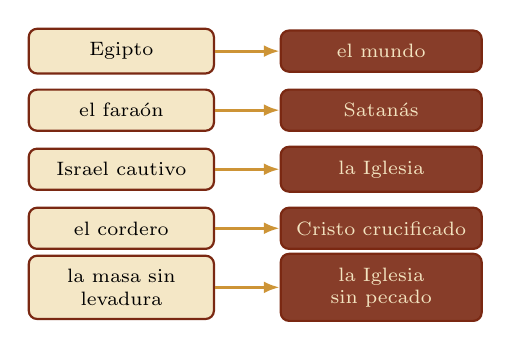
\begin{tikzpicture}[font=\scriptsize]
 \foreach \y/\a/\b in {0/Egipto/el mundo, -0.75/el faraón/Satanás, -1.5/Israel cautivo/la Iglesia, -2.25/el cordero/Cristo crucificado, -3.0/la masa sin levadura/la Iglesia sin pecado}{
  \node[caja,text width=2.0cm,align=center] (x) at (0,\y) {\a};
  \node[caja,text width=2.2cm,align=center,fill=tierraroja,text=papiro] (z) at (3.3,\y) {\b};
  \draw[-{Latex[length=2mm]},mostaza!90!tierraroja,line width=1pt] (x)--(z);}
\end{tikzpicture}
\end{column}
\begin{column}{0.48\textwidth}
\begin{cita}\ldots{}cuando estabais muertos en vuestros delitos y pecados\ldots{} conforme al príncipe de la potestad del aire\ldots\fuente{(Ef 2:1--2, RVR1960)}\end{cita}
\scriptsize Apoyos: 1 Co 10:1--11 (\grc{τύποι}); Col 1:13; He 2:14--15; Ez 29:3 (el faraón, ``gran dragón''); Ap 12:9.\par
\precision{lectura tipológica de la serie; ningún texto dice ``el faraón es Satanás''.}
\end{column}
\end{columns}
\end{frame}

\begin{frame}{La observancia apostólica}
\small
\begin{itemize}
\item \destacar{Hch 12:3}: ``Eran entonces los días de los panes sin levadura''. La serie: Herodes sabía que la Iglesia guardaría esos días.\\
\precision{Lucas fecha el arresto y da como motivo agradar a los judíos (12:3--4).}
\item \destacar{Hch 20:6}: ``pasados los días de los panes sin levadura, navegamos de Filipos''. Pablo espera el fin de la semana (Longenecker, 1981).
\item \destacar{1 Co 5:8}: ``celebremos la fiesta''. Para la serie, la misma fiesta instituida por Dios, guardada por judíos y gentiles en Corinto (Iglesia de Dios Unida, 2011).
\end{itemize}
\end{frame}

\begin{frame}{\emph{Bedikat jamets}: la casa de Dios}
\begin{columns}[t,onlytextwidth]
\begin{column}{0.48\textwidth}\small
\destacar{La práctica}: antes de la Pascua se busca la levadura en cada rincón de la casa ``a la luz de una lámpara'' (Pesajim 1:1).\par\medskip
\destacar{La aplicación} (presentación de Danilo): los creyentes son la casa de Dios:
\begin{itemize}
\item ``la cual casa somos nosotros'' (He 3:6); ``casa espiritual'' (1 P 2:5);
\item ``casa de Dios, que es la iglesia'' (1 Ti 3:15; Ef 2:19);
\item el cuerpo, templo del Espíritu (1 Co 3:16--17; 6:19--20; 2 Co 6:16).
\end{itemize}
\end{column}
\begin{column}{0.50\textwidth}
\begin{tcolorbox}[colback=papiro,colframe=tierraroja,boxrule=1pt,arc=3pt]
\small\centering Si la casa de Israel debía quedar sin \emph{se'or} (Éx 12:15), la casa de Dios debe quedar \destacar{sin la levadura del pecado}.
\end{tcolorbox}
\precision{la búsqueda con lámpara es tradición rabínica; la imagen de la casa de Dios es de la Escritura.}
\end{column}
\end{columns}
\end{frame}

\begin{frame}{Cómo celebrarla hoy}
\begin{columns}[t,onlytextwidth]
\begin{column}{0.50\textwidth}\small
\begin{itemize}
\item ``Con panes sin levadura, de \destacar{sinceridad y de verdad}'' (1 Co 5:8): pureza, santidad, separación.
\item El lavamiento: ``ya habéis sido lavados'' (1 Co 6:11); ``bautízate, y lava tus pecados'' (Hch 22:16).
\item Israel ``bautizado en la nube y en el mar'' después de la Pascua (1 Co 10:1--2).
\item Sumergirse en la Palabra.
\end{itemize}
\end{column}
\begin{column}{0.48\textwidth}\scriptsize
\destacar{El ``gran sábado''}: el 15 de Nisán es día de reposo propio de la semana (Lv 23:7; Jn 19:31).\par\medskip
\precision{la presentación de Danilo reúne en el 17 de Nisán el arca en el Ararat (Gn 8:4, ``mes séptimo'' leído en calendario civil), el cruce del mar, el primer fruto de la tierra y la caída de Amán. Son cómputos tradicionales: Jos 5:11 dice ``al otro día de la pascua'' (el 15) y el cruce no tiene fecha en el texto.}
\end{column}
\end{columns}
\end{frame}

% ------------------------------------------------------------------
\section{Mesías}

\begin{frame}{``Yo soy el pan de vida''}
\begin{columns}[t,onlytextwidth]
\begin{column}{0.52\textwidth}
\centering\grc{ἐγώ εἰμι ὁ ἄρτος τῆς ζωῆς}
\begin{cita}Yo soy el pan de vida; el que a mí viene, nunca tendrá hambre; y el que en mí cree, no tendrá sed jamás.\fuente{(Jn 6:35, RVR1960)}\end{cita}
\end{column}
\begin{column}{0.46\textwidth}\small
\begin{itemize}
\item ``Estaba cerca la pascua'' (Jn 6:4).
\item Comida en el desierto, paso del mar, pan del cielo: un \destacar{éxodo}.
\item ``El pan que yo daré es mi carne\ldots{} por la vida del mundo'' (6:51).
\end{itemize}
\end{column}
\end{columns}
\end{frame}

\begin{frame}{``Esto es mi cuerpo''}
\begin{columns}[t,onlytextwidth]
\begin{column}{0.50\textwidth}
\begin{cita}Y tomó el pan y dio gracias, y lo partió y les dio, diciendo: Esto es mi cuerpo, que por vosotros es dado; haced esto en memoria de mí.\fuente{(Lc 22:19, RVR1960)}\end{cita}
\small ``En memoria'' retoma Éx 12:14 (Jeremias, 1966).
\end{column}
\begin{column}{0.48\textwidth}\scriptsize
\begin{itemize}
\item Sinópticos: cena pascual (Mc 14:12--16) $\Rightarrow$ pan sin levadura.
\item Juan: crucifixión en la ``preparación de la pascua'' (Jn 18:28; 19:14).
\item \grc{ἄρτος} es término general (LXX \grc{ἄρτους ἀζύμους}, Éx 29:2).
\end{itemize}
\precision{la fecha de la cena es discutida; la controversia ázimos/pan leudado (s.~\textsc{xi}) es historia posterior.}
\end{column}
\end{columns}
\end{frame}

\begin{frame}{Sepultado al comenzar los ázimos}
\begin{columns}[t,onlytextwidth]
\begin{column}{0.52\textwidth}
\begin{cita}\ldots{}a fin de que los cuerpos no quedasen en la cruz en el día de reposo (pues aquel día de reposo era de gran solemnidad)\ldots\fuente{(Jn 19:31, RVR1960)}\end{cita}
\small El ``gran'' sábado: el \destacar{15 de Nisán}, primer día santo. El ``grano de trigo'' en tierra (Jn 12:24).
\end{column}
\begin{column}{0.46\textwidth}\scriptsize
\precision{el día de la semana se discute: viernes (tradición mayoritaria) o miércoles (algunos materiales del proyecto, por Mt 12:40). La \emph{matsá} ``rayada y perforada'' (Is 53:5; Zac 12:10) y el \emph{afikomán} son lecturas devocionales de prácticas posteriores.}
\end{column}
\end{columns}
\end{frame}


% ------------------------------------------------------------------
\section{Tradición}

\begin{frame}{La fiesta en la tradición judía}
\begin{columns}[t,onlytextwidth]
\begin{column}{0.50\textwidth}\scriptsize
\begin{itemize}
\item \destacar{\emph{Bedikat jamets}}: búsqueda la noche del 14 ``a la luz de una lámpara'' (Pesajim 1:1).
\item \destacar{\emph{Biur}}: quema del \emph{jamets} (1:4; 2:1).
\item Cinco cereales para la \emph{matsá} (2:5); ``18 minutos'' (de Pesajim 46a).
\item \emph{Matsá shemurá}: ``vigilaréis las \emph{matsot}'' (Éx 12:17).
\end{itemize}
\end{column}
\begin{column}{0.48\textwidth}\scriptsize
\begin{itemize}
\item Gamaliel: Pésaj, \emph{matsá}, \emph{maror} (Pesajim 10:5).
\item 7.º día: Cántico del Mar (Meguilá 31a).
\item 8.º día en la diáspora.
\item ``La levadura de la masa'' como impulso al mal (Berajot 17a).
\end{itemize}
\end{column}
\end{columns}\medskip
\precision{todo esto es tradición rabínica posterior (Misná ca. 200 e.\,c.; Talmud); el Séder actual es más tardío (Bokser, 1984).}
\end{frame}

% ------------------------------------------------------------------
\section{Discusión}

\begin{frame}{1 Co 5:8: ¿mandato o metáfora?}
\scriptsize\renewcommand{\arraystretch}{1.15}
\begin{tabular}{@{}L{2.6cm}L{6.0cm}L{3.4cm}@{}}
\toprule
\textbf{Lectura} & \textbf{Argumentos} & \textbf{Autores} \\ \midrule
Metáfora de la vida cristiana & contexto disciplinario; presente continuo: toda la vida es la fiesta & Fee (1987); Thiselton (2000) \\
Observancia con sentido nuevo & escrita cerca de Pascua (16:8); la imagen supone la práctica; Hch 20:6 & Bacchiocchi (1995); IDU (2011); serie \\
Combinada & la metáfora nace de una práctica viva, sin legislar en el pasaje & Hays (1997) \\
\bottomrule
\end{tabular}\par\medskip
\small Común a todas: la fiesta tiene su sentido pleno en \destacar{Cristo, nuestra Pascua}, y se celebra con una vida sin malicia.
\end{frame}


% ------------------------------------------------------------------
\section{Síntesis}

\begin{frame}{Definición}
\begin{tcolorbox}[colback=papiro,colframe=tierraroja,boxrule=1pt,arc=3pt]
\small La fiesta de los Panes sin Levadura (\heb{חַג הַמַּצּוֹת}; \grc{ἑορτὴ τῶν ἀζύμων}) es la convocación del \SENOR{} del \destacar{15 al 21 de Abib}, con el primero y el séptimo día santos, en que Israel come \emph{matsot} y quita toda \emph{se'or} y \emph{jamets}, ``porque en este mismo día saqué vuestras huestes'' (Éx 12:17). Memorial de la salida (Dt 16:3) y, en el Nuevo Testamento, imagen de la comunidad que vive como ``nueva masa, sin levadura'' porque ``nuestra pascua, que es Cristo, ya fue sacrificada'' (1 Co 5:7--8).
\end{tcolorbox}
\end{frame}

\begin{frame}{Lectura y aporte}
\scriptsize\renewcommand{\arraystretch}{1.13}
\begin{tabular}{@{}L{2.0cm}L{10.0cm}@{}}
\toprule
Histórica & la salida de prisa; pan de pobres y caminantes; la fiesta en Gilgal, Ezequías, Josías, Esdras, Elefantina, Josefo \\
Filológica & \emph{se'or}, \emph{jamets}, \emph{matsá}; \emph{lejem oni}; \emph{tsiv'ot}; de \emph{ázyma} a \emph{ázymoi} \\
Textual & el ``primer día'', los ``seis días'', \emph{matsot/mitsvá}, Mc 14:12; levadura fuera del altar, no de la mesa \\
Literaria & semana entre dos días santos; ley incrustada en el relato; levadura negativa y positiva \\
De la serie & memorial de Israel libre del cautiverio; la Iglesia sin levadura, libre de Satanás; Hch 12:3; 20:6 \\
En Cristo & pan de vida (Jn 6:35); el pan de la cena; sepultado al comenzar los ázimos; 1 Co 5:7 \\
\bottomrule
\end{tabular}
\end{frame}

% ------------------------------------------------------------------
\section{Reflexión}

\begin{frame}{Para la reflexión}
\small
\begin{enumerate}
\item Israel comió \emph{matsot} \destacar{porque} salió, no \destacar{para} salir. ¿Qué cambia si la limpieza es consecuencia de la Pascua (1 Co 5:7)?
\item ¿Cuáles son las ``masas madre'' que, guardadas, fermentan cada nueva amasada de la vida?
\item ¿Qué levadura tolera hoy una iglesia por ``jactancia'' (1 Co 5:6)?
\item ``Lo contarás en aquel día a tu hijo'' (Éx 13:8): ¿cómo se transmite el relato de la liberación?
\item ¿Dónde crece, escondida, la levadura buena del reino (Mt 13:33)?
\end{enumerate}
\end{frame}

% ------------------------------------------------------------------
\section{Glosario}

\begin{frame}{Glosario}
\scriptsize
\begin{columns}[t,onlytextwidth]
\begin{column}{0.49\textwidth}
\textbf{Abib} (\heb{אָבִיב}): ``espiga verde''; primer mes.\\
\textbf{\emph{Ázyma}} (\grc{ἄζυμα}): ázimos; la fiesta.\\
\textbf{\emph{Atséret}} (\heb{עֲצֶרֶת}): asamblea de clausura.\\
\textbf{\emph{Bedikat jamets}}: búsqueda de la levadura (tradición).\\
\textbf{\emph{Biur}}: quema de la levadura (tradición).\\
\textbf{\emph{Eilikríneia}} (\grc{εἰλικρίνεια}): sinceridad.\\
\textbf{\emph{Jamets}} (\heb{חָמֵץ}): lo leudado.\\
\textbf{\emph{Karet}} (\heb{כָּרֵת}): ``ser cortado''.\\
\textbf{\emph{Lejem oni}} (\heb{לֶחֶם עֹנִי}): pan de aflicción.
\end{column}
\begin{column}{0.49\textwidth}
\textbf{\emph{Majméset}} (\heb{מַחְמֶצֶת}): cualquier cosa leudada.\\
\textbf{\emph{Matsá}} (\heb{מַצָּה}): torta sin leudar.\\
\textbf{\emph{Mikrá kódesh}} (\heb{מִקְרָא קֹדֶשׁ}): santa convocación.\\
\textbf{\emph{Phýrama}} (\grc{φύραμα}): masa.\\
\textbf{\emph{Se'or}} (\heb{שְׂאֹר}): masa madre.\\
\textbf{\emph{Tsiv'ot}} (\heb{צִבְאוֹת}): huestes.\\
\textbf{\emph{Yam Suf}} (\heb{יַם־סוּף}): mar de juncos.\\
\textbf{\emph{Zýmē}} (\grc{ζύμη}): levadura.
\end{column}
\end{columns}
\end{frame}

% ------------------------------------------------------------------
\section{Referencias}

\begin{frame}{Referencias (1)}
\fontsize{6}{7.2}\selectfont
\refapa{Bacchiocchi, S. (1995). \emph{God's festivals in Scripture and history: Part 1. The spring festivals}. Biblical Perspectives.}
\refapa{Bokser, B. M. (1984). \emph{The origins of the Seder}. University of California Press.}
\refapa{Brown, F., Driver, S. R., \& Briggs, C. A. (1906). \emph{A Hebrew and English lexicon of the Old Testament}. Clarendon.}
\refapa{Davies, W. D., \& Allison, D. C. (1991). \emph{Matthew} (Vol. 2, ICC). T\&T Clark.}
\refapa{de Vaux, R. (1985). \emph{Instituciones del Antiguo Testamento}. Herder.}
\refapa{Elliger, K., \& Rudolph, W. (Eds.). (1997). \emph{Biblia Hebraica Stuttgartensia} (5.ª ed.). Deutsche Bibelgesellschaft.}
\refapa{Fee, G. D. (1987). \emph{The first epistle to the Corinthians} (NICNT). Eerdmans.}
\refapa{Hagner, D. A. (1993). \emph{Matthew 1--13} (WBC 33A). Word.}
\refapa{Hays, R. B. (1997). \emph{First Corinthians} (Interpretation). John Knox.}
\refapa{Hoffmeier, J. K. (1997). \emph{Israel in Egypt}. Oxford University Press.}
\refapa{Iglesia de Dios Unida. (2011). \emph{Las fiestas santas de Dios: esperanza segura para toda la humanidad}.}
\refapa{Jeremias, J. (1966). \emph{The eucharistic words of Jesus}. SCM.}
\refapa{Josefo, F. (1997). \emph{Antigüedades judías} (J. Vara Donado, Trad.). Akal.}
\refapa{Kitchen, K. A. (2003). \emph{On the reliability of the Old Testament}. Eerdmans.}
\refapa{Koehler, L., \& Baumgartner, W. (2001). \emph{HALOT}. Brill.}
\end{frame}

\begin{frame}{Referencias (2)}
\fontsize{6}{7.2}\selectfont
\refapa{Longenecker, R. N. (1981). Acts. En F. E. Gaebelein (Ed.), \emph{The expositor's Bible commentary} (Vol. 9). Zondervan.}
\refapa{Milgrom, J. (1991). \emph{Leviticus 1--16} (AB 3). Doubleday.}
\refapa{Milgrom, J. (2001). \emph{Leviticus 23--27} (AB 3B). Doubleday.}
\refapa{Nestle, E., \& Aland, K. (2012). \emph{Novum Testamentum Graece} (28.ª ed.). Deutsche Bibelgesellschaft.}
\refapa{Pentecost, J. D. (1958). \emph{Things to come}. Dunham.}
\refapa{Porten, B. (1968). \emph{Archives from Elephantine}. University of California Press.}
\refapa{Propp, W. H. C. (1999). \emph{Exodus 1--18} (AB 2). Doubleday.}
\refapa{Rahlfs, A., \& Hanhart, R. (Eds.). (2006). \emph{Septuaginta}. Deutsche Bibelgesellschaft.}
\refapa{\emph{Santa Biblia Reina-Valera 1960}. (1960). Sociedades Bíblicas en América Latina.}
\refapa{Scofield, C. I. (Ed.). (1909). \emph{The Scofield reference Bible}. Oxford University Press.}
\refapa{Sefaria. (s.f.). Misná \emph{Pesajim}; Talmud; Rashi. https://www.sefaria.org}
\refapa{Thiselton, A. C. (2000). \emph{The first epistle to the Corinthians} (NIGTC). Eerdmans.}
\refapa{Tigay, J. H. (1996). \emph{Deuteronomy} (JPS). Jewish Publication Society.}
\refapa{Wenham, G. J. (1979). \emph{The book of Leviticus} (NICOT). Eerdmans.}
\refapa{Wight, F. H. (1953). \emph{Usos y costumbres de las tierras bíblicas}. Portavoz.}
\refapa{Yadin, Y. (1983). \emph{The Temple Scroll}. Israel Exploration Society.}\par\smallskip
{\color{sepia}Citas bíblicas: Reina-Valera 1960 (\SENOR{} por ``Jehová''); hebreo BHS; griego NA28 y LXX Rahlfs-Hanhart. Imágenes y diagramas: elaboración propia.}
\end{frame}

\end{document}
